\documentclass{beamer}
\usepackage{etex}
\usepackage[utf8]{inputenc}
\usepackage[T1]{fontenc}
\usepackage[francais]{babel}
\usepackage{amssymb}
\usepackage{epsfig,shadow}
\usepackage{verbatim}
\usepackage{pstricks}
\usepackage{beamerthemesplit}
\usepackage{graphicx}
%\usepackage{comment}
\usepackage{algorithm}
\usepackage{listings}
\usepackage{figlatex}
\usepackage[french]{algorithmic}
\usepackage{multirow}

\graphicspath{{fig/}{campagne/fig}}
\newcommand{\talk}[2]{{#1} dit : {#2}}
\newcommand{\erik}[1]{\talk{Erik}{#1}}
\newcommand{\brice}[1]{\talk{Brice}{#1}}
\beamertemplatetransparentcovereddynamic

%\setbeamertemplate{background canvas}[vertical shading][bottom=red!10,top=blue!10]
%\usetheme{Warsaw}

\usecolortheme{progressbar}
\usefonttheme{progressbar}
\useoutertheme{progressbar}
\useinnertheme{progressbar}

\newcommand{\bordereau}{Bordereau\xspace}
\newcommand{\genepi}{Genepi\xspace}
\newcommand{\minelement}{{\em min\_element}\xspace}
\newcommand{\stablesort}{{\em stable\_sort}\xspace}
\newcommand{\merge}{{\em merge}\xspace}
\newcommand{\sort}{{\em sort}\xspace}
\newcommand{\find}{{\em find}\xspace}
\setbeamertemplate{navigation symbols}{}
\beamertemplatetransparentcovereddynamic
\newcommand{\pastel}{PaSTeL\xspace}

\definecolor{javared}{rgb}{0.6,0,0} % for strings
\definecolor{javagreen}{rgb}{0.25,0.5,0.35} % comments
\definecolor{javapurple}{rgb}{0.5,0,0.35} % keywords
\definecolor{javadocblue}{rgb}{0.25,0.35,0.75} % java


\title{BOAST}
\subtitle{Porting HPC applications to the Mont-Blanc prototype using BOAST }
\author{Kevin Pouget, \textbf{Brice Videau}, Jean-François Méhaut\\
(INRIA Grenoble - LIG - NANOSIM)}

\date{\textbf{Tutorial BOAST}\\September 19, 2014}

\begin{document}

\frame{\titlepage}

\section{Introduction}

\frame{
    \frametitle{Introduction}
}

\subsection{Context}

\begin{frame}
    \frametitle{Scientific Application Optimization}
\begin{itemize}
\item In the past, waiting for a new generation of hardware was enough to obtain performance gains.
\item Nowadays, architecture are so different that performance regress when a new architecture is released.
\item Sometimes the code is not fit anymore and cannot be compiled.
\item Few applications can harness the power of current computing platforms.
\item Thus, optimizing scientific application is of paramount importance.
\end{itemize}
\end{frame}

\begin{frame}
\frametitle{Multiplicity of Architectures}
A High performance Computing application can encounter several types of architectures:
\begin{itemize}
\item Generalist Multicore CPU (AMD, Intel, PowerPC...)
\item Graphical Accelerators (ATI, NVIDIA...)
\item Computing Accelerators (CELL, MIC...)
\item \textbf{Low power CPUs (ARM...)}
\end{itemize}
Those architectures can present drastically different characteristics.
\end{frame}

\begin{frame}
\frametitle{Architectures Comparison}
\begin{table}
\centering
\footnotesize
\begin{tabular}{|l|r|r|r|r|}
\hline
Architecture & AMD/Intel CPUs & ARM & GPUs & Xeon Phi \\
\hline
Cores    & 4-12   & 2-4   & 512-2496    & 60  \\
\hline
Cache    & 3l & 2l & 2l incoherent & 2l \\
\hline
Memory (GiB)   & 2-4 (per core)   & 1 (per core)   & 2-6    & 6-16   \\
\hline
Vector Size   & 2-4    & 1-2    & 1-2    & 8 \\
\hline
Peak GFLOPS & 10-20 (per core)    & 2-4 (per core)   & 500-1500    & 1000\\
\hline
Peak GiB/s & 20-40 & 2.5-5 & 150-250 & 200\\
\hline
TDP W & 75  & 5 & 200 & 300\\
\hline
GFLOPS/W & 1-3 & 2-4 & 2-7 & 3\\
\hline
\end{tabular} \caption{Comparison between commonly found architectures in HPC.}
\end{table}
\end{frame}

\subsection{Problematic}

\begin{frame}
\frametitle{Exploiting Various Architectures}
Usually work is done on a class of architecture (CPUs or GPUs or accelerators).\\
\begin{block}{Well Known Examples}
\begin{itemize}
\item Atlas (Linear Algebra CPU)
\item PhiPAC (Linear Algebra CPU)
\item Spiral (FFT CPU)
\item FFTW (FFT CPU)
\item NukadaFFT(FFT GPU)
\end{itemize}
\end{block}
No work targeting several class of architectures.
What if the application is not based on a library?
\end{frame}


\subsection{Use Cases}

\begin{frame}
\frametitle{The Mont-Blanc European Project}
\begin{center}

\includegraphics[scale=0.3]{Mont-Blanc_logo-horizontal}
\end{center}
European project:
\begin{itemize}
\item Develop prototypes of HPC clusters using low power commercially available embedded technology (ARM CPUs, low power GPUs...).
\item Design the next generation in HPC systems based on embedded technologies and experiments on the prototypes.
\item Develop a portfolio of existing applications to test these systems and optimize their efficiency, using BSC's OmpSs programming model (11 existing applications were selected for this portfolio).
\end{itemize}
Prototype : based on Exynos 5250 : dual core Cortex A15 with T604 Mali GPU (OpenCL)
\end{frame}

\begin{frame}
    \frametitle{BigDFT a Tool for Nanotechnologies}
\begin{columns}
\column{6cm}
Ab initio simulation:
\begin{itemize}
  \item Simulates the properties of crystals and molecules,
  \item Computes the electronic density,
  \item Based on Daubechie wavelet.
\end{itemize}
The formalism was chosen because it is fit for HPC computations: 
\begin{itemize}
\item Each orbital can be treated independently most of the time,
\item Operator on orbitals are simple and straightforward.
\end{itemize}
\column{4.5cm}
\centering
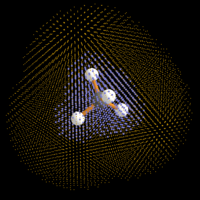
\includegraphics[width=3.5cm]{CH4-grid.png}\\
Electronic density around a methane molecule.
\end{columns}
\end{frame}

\begin{frame}
\frametitle{BigDFT as an HPC application}
\begin{block}{Implementation details:}
\begin{itemize}
\item 200,000 lines of Fortran 90 and C
\item Supports MPI, OpenMP, CUDA and OpenCL
\item Uses BLAS
\item Scalability up to 16000 cores of Curie and 288GPUs
\end{itemize}
\end{block}

\begin{block}{Operators can be expressed as 3D convolutions:}
  \begin{itemize}
    \item Wavelet Transform
    \item Potential Energy
    \item Kinetic Energy
  \end{itemize}
  These convolutions are separable and filter are short (16 elements).\\
  Can take up to 90\% of the computation time on some systems.
\end{block}
\end{frame}

\begin{frame}
  \frametitle{SPECFEM3D a tool for wave propagation research}
\begin{columns}
\column{6cm}
Wave propagation simulation:
\begin{itemize}
  \item Used for geophysics and material research,
  \item Accurately simulate earthquakes,
  \item Based on spectral finite element.
\end{itemize}
Developped all around the world:
\begin{itemize}
\item Marseilles (CNRS),
\item Switzerland (ETH Zurich) CUDA,
\item United States (Princeton) Networking,
\item Grenoble (LIG/CNRS) OpenCL.
\end{itemize}
\column{5cm}
\centering
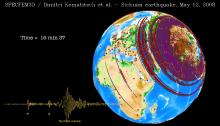
\includegraphics[width=5cm]{image_movie_Sichuan_009000_0.jpg}\\
Sichuan earthequake.
\end{columns}
\end{frame}

\begin{frame}
\frametitle{SPECFEM3D as an HPC application}
\begin{block}{Implementation details:}
\begin{itemize}
\item 80,000 lines of Fortran 90
\item Supports MPI, CUDA, OpenCL and an OMPSs + MPI miniapp
\item Scalability up to 693,600 cores on IBM BlueWaters
\end{itemize}
\end{block}
\end{frame}


\begin{frame}
    \frametitle{Talk Outline}
    \tableofcontents[hideallsubsections,sections={2-}]
    %\includegraphics{plan_couleur.pdf}
\end{frame}

\section{Case Study}


\begin{frame}[fragile]
\frametitle{Case Study 1: BigDFT's MagicFilter}
The simplest convolution found in BigDFT, corresponds to the potential operator.
\begin{columns}
\column{4cm}
\begin{block}{Characteristics}
\begin{itemize}
\item Separable,
\item Filter length 16,
\item Transposition,
\item Periodic,
\item Only 32 operations per element.
\end{itemize}
\end{block}
\column{6.2cm}
\begin{block}{Pseudo code}
\tiny
\lstset{language=C,numbers=left}
\begin{lstlisting}
double filt[16] = {F0, F1, ... , F15};
void magicfilter(int n, int ndat, 
                 double *in, double *out){
  double temp;
  for(j=0; j<ndat; j++) {
    for(i=0; i<n; i++) {
       temp = 0;
       for(k=0; k<16; k++) {
         temp+= in[ ((i-7+k)%n) + j*n] 
                  * filt[k];
       }
       out[j + i*ndat] = temp;
} } }
\end{lstlisting}
\end{block}
\end{columns}
\end{frame}

\begin{frame}
\frametitle{Case study 2: SPECFEM3D port to OpenCL}
\begin{block}{Existing CUDA code:}
\begin{itemize}
\item 42 kernels and 15000 lines of code
\item kernels with 80+ parameters
\item $\sim{}$ 7500 lines of cuda code
\item $\sim{}$ 7500 lines of wrapper code
\end{itemize}
\end{block}
\begin{block}{Objectives:}
\begin{itemize}
\item Factorize the existing code,
\item Single OpenCL and CUDA description for the kernels,
\item Validate without unit tests, comparing native Cuda to generated Cuda executions
\item Keep similar performances.
\end{itemize}
\end{block}
\end{frame}

\section{A Parametrized Generator}
\begin{frame}
\frametitle{A Parametrized Generator}
\end{frame}

\begin{frame}
\frametitle{Classical Workflow}
\begin{figure}
\centering
\includegraphics<1>[scale=1]{Workflow1-1}
\includegraphics<2>[scale=1]{Workflow1-2}
\includegraphics<3>[scale=1]{Workflow1-3}
\includegraphics<4>[scale=1]{Workflow1-4}
\label{fig:2filters}
\end{figure}
\begin{itemize}
\item<1|only@1> Kernel optimization workflow
\item<1|only@1> Usually performed by a knowledgeable developer
\item<2|only@2> Compilers perform optimizations
\item<2|only@2> Architecture specific or generic optimizations
\item<3|only@3> Performance data hint at source transformations
\item<3|only@3> Architecture specific or generic hints
\item<4|only@4> Multiplication of kernel versions or loss of versions
\item<4|only@4> Difficulty to benchmark versions against each-other
\end{itemize}
\end{frame}

\begin{frame}
\frametitle{BOAST Workflow}
\begin{figure}
\centering
\includegraphics<1>[scale=1]{Workflow2-1}
\includegraphics<2>[scale=1]{Workflow2-2}
\includegraphics<3>[scale=1]{Workflow2-3}
\label{fig:2filters}
\end{figure}
\begin{itemize}
\item<1|only@1> Meta-programming of optimizations in BOAST
\item<1|only@1> High level object oriented language
\item<2|only@2> Generate combination of optimizations
\item<2|only@2> C, OpenCL, FORTRAN and CUDA are supported
\item<3|only@3> Compilation and analysis are automated
\item<3|only@3> Selection of best version can also be automated
\end{itemize}
\end{frame}

\begin{frame}
\frametitle{BOAST}
\begin{figure}
\centering
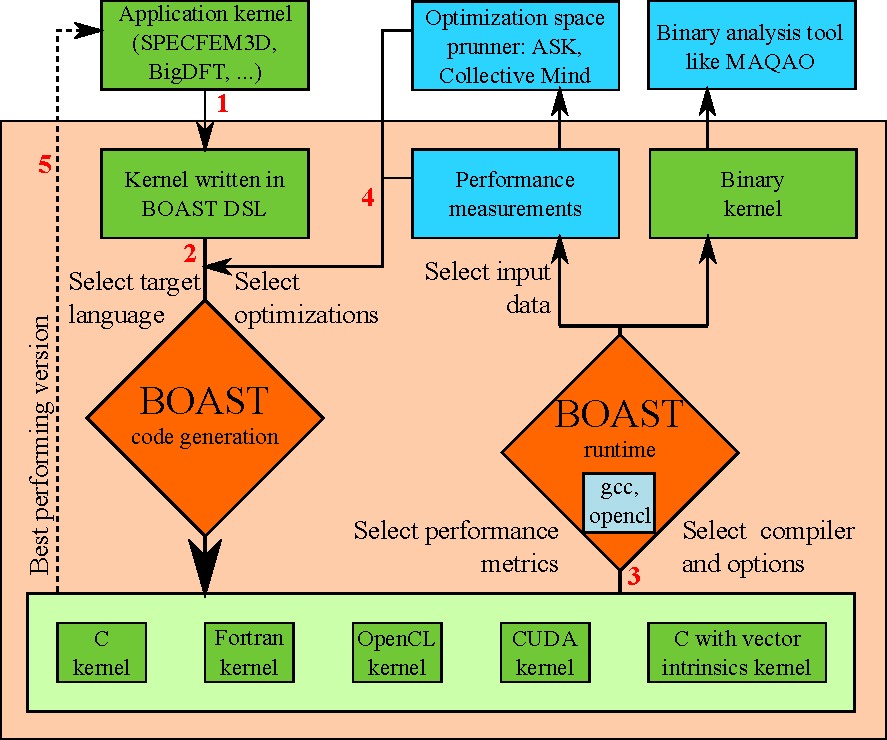
\includegraphics[scale=0.5]{BOAST}
\end{figure}
\end{frame}

\begin{frame}
\frametitle{Use Case Driven}
Parameters arising in a convolution:
\begin{itemize}
\item Filter: length, values, center.
\item Direction: forward or inverse convolution.
\item Boundary conditions: free or periodic.
\item Unroll factor: arbitrary.
\end{itemize}
How are those parameters constraining our tool?
\end{frame}

\begin{frame}
\frametitle{Features required}
Unroll factor:
\begin{itemize}
\item Create and manipulate an unknown number of variables,
\item Create loops with variable steps.
\end{itemize}
Boundary conditions:
\begin{itemize}
\item Manage arrays with parametrized size.
\end{itemize}
Filter and convolution direction:
\begin{itemize}
\item Transform arrays.
\end{itemize}
And of course be able to describe convolutions and output them in different languages.
\end{frame}

\begin{frame}
\frametitle{Proposed Generator}
Idea: use a high level language with support for operator overloading to describe the structure of the code, rather than trying to transform a decorated tree.\\
Define several abstractions:
\begin{itemize}
\item Variables: type (array, float, integer), size...
\item Operators: affect, multiply...
\item Procedure and functions: parameters, variables...
\item Constructs: for, while...
\end{itemize}
\end{frame}

\begin{frame}[fragile]
\frametitle{Sample Code: Variables and Parameters}
\tiny
%\lstset{language=Ruby,numbers=left}
\lstset{language=Ruby,
basicstyle=\ttfamily,
keywordstyle=\color{javapurple}\bfseries,
stringstyle=\color{javared},
commentstyle=\color{javagreen},
numbers=left,
tabsize=4,
showspaces=false,
showstringspaces=false}
\begin{lstlisting}
  #simple Variable
  i = Int "i"
  #simple constant
  lowfil = Int( "lowfil", :const => 1-center )
  #simple constant array
  fil = Real("fil", :const => arr, :dim => [ Dim(lowfil,upfil) ])
  #simple parameter
  ndat = Int("ndat", :dir => :in)
  #multidimensional array, an output parameter
  y = Real("y", :dir => :out, :dim => [ Dim(ndat), Dim(dim_out_min, dim_out_max) ] )
\end{lstlisting}
\normalsize
Variables and Parameters are objects with a name, a type, and a set of named properties.
\end{frame}

\begin{frame}[fragile]
\frametitle{Sample Code: Procedure Declaration}
The following declaration:
\tiny
\lstset{language=Ruby,
basicstyle=\ttfamily,
keywordstyle=\color{javapurple}\bfseries,
stringstyle=\color{javared},
commentstyle=\color{javagreen},
numbers=left,
tabsize=4,
showspaces=false,
showstringspaces=false}
\begin{lstlisting}
p = Procedure("magic_filter", [n,ndat,x,y], [lowfil,upfil])
opn p
\end{lstlisting}
\normalsize 
Outputs Fortran:
\tiny
\lstset{language=Fortran,
basicstyle=\ttfamily,
keywordstyle=\color{javapurple}\bfseries,
stringstyle=\color{javared},
commentstyle=\color{javagreen},
numbers=left,
tabsize=4,
showspaces=false,
showstringspaces=false}
\begin{lstlisting}
subroutine magicfilter(n, ndat, x, y)
  integer(kind=4), parameter :: lowfil = -8
  integer(kind=4), parameter :: upfil = 7
  integer(kind=4), intent(in) :: n
  integer(kind=4), intent(in) :: ndat
  real(kind=8), intent(in), dimension(0:n-1, ndat) :: x
  real(kind=8), intent(out), dimension(ndat, 0:n-1) :: y
\end{lstlisting}
\normalsize
Or C:
\tiny
\lstset{language=C,
basicstyle=\ttfamily,
keywordstyle=\color{javapurple}\bfseries,
stringstyle=\color{javared},
commentstyle=\color{javagreen},
numbers=left,
tabsize=4,
showspaces=false,
showstringspaces=false}
\begin{lstlisting}
void magicfilter(const int32_t n, const int32_t ndat, const double * x, double * y){
  const int32_t lowfil = -8;
  const int32_t upfil = 7;
\end{lstlisting}
\end{frame}

\begin{frame}[fragile]
\frametitle{Sample Code: Constructs and Arrays}
The following declaration:
\tiny
\lstset{language=Ruby,
basicstyle=\ttfamily,
keywordstyle=\color{javapurple}\bfseries,
stringstyle=\color{javared},
commentstyle=\color{javagreen},
numbers=left,
tabsize=4,
showspaces=false,
showstringspaces=false}
\begin{lstlisting}
  unroll = 5
  pr For(j,1,ndat-(unroll-1), unroll) {
  #.....
    pr tt2 === tt2 + x[k,j+1]*fil[l]
  #.....
  }
\end{lstlisting}
\normalsize 
Outputs Fortran:
\tiny
\lstset{language=Fortran,
basicstyle=\ttfamily,
keywordstyle=\color{javapurple}\bfseries,
stringstyle=\color{javared},
commentstyle=\color{javagreen},
numbers=left,
tabsize=4,
showspaces=false,
showstringspaces=false}
\begin{lstlisting}
  do j=1, ndat-4, 5
    !......
    tt2=tt2+x(k,j+1)*fil(l)
    !......
  enddo
\end{lstlisting}
\normalsize
Or C:
\tiny
\lstset{language=C,
basicstyle=\ttfamily,
keywordstyle=\color{javapurple}\bfseries,
stringstyle=\color{javared},
commentstyle=\color{javagreen},
numbers=left,
tabsize=4,
showspaces=false,
showstringspaces=false}
\begin{lstlisting}
  for(j=1; j<=ndat-4; j+=5){
  /*...........*/
    tt2=tt2+x[k-0+(j+1-1)*(n-1-0+1)]*fil[l-lowfil];
  /*...........*/
  }
\end{lstlisting}
\end{frame}

\section{Evaluation}
\begin{frame}
\frametitle{Generator Evaluation}
Back to the test cases:
\begin{itemize}
\item The generator was used to unroll the Magicfilter an evaluate it's performance on an ARM processor and an Intel processor.
\item The generator was used to describe SPECFEM3D kernel.
\end{itemize}

\end{frame}

\begin{frame}
\frametitle{Performance Results}
\centering
\begin{columns}
\column{5cm}
\begin{block}{Tegra2}
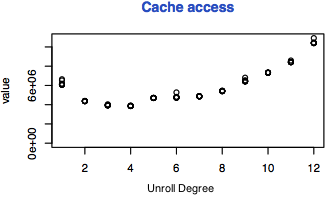
\includegraphics[scale=0.4]{cacc}\\
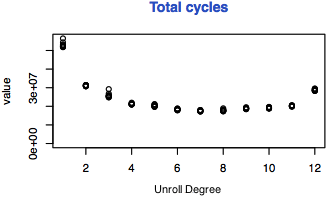
\includegraphics[scale=0.4]{totcyc}
\end{block}
\column{5cm}
\begin{block}{Intel T7500}
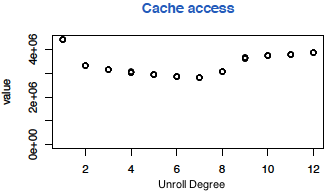
\includegraphics[scale=0.4]{nedni_cacc.png}\\
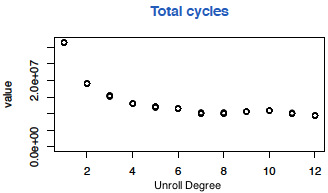
\includegraphics[scale=0.4]{nedni_totcyc.png}
\end{block}
\end{columns}
\end{frame}

\begin{frame}
\frametitle{BigDFT Synthesis Kernel}
\centering 
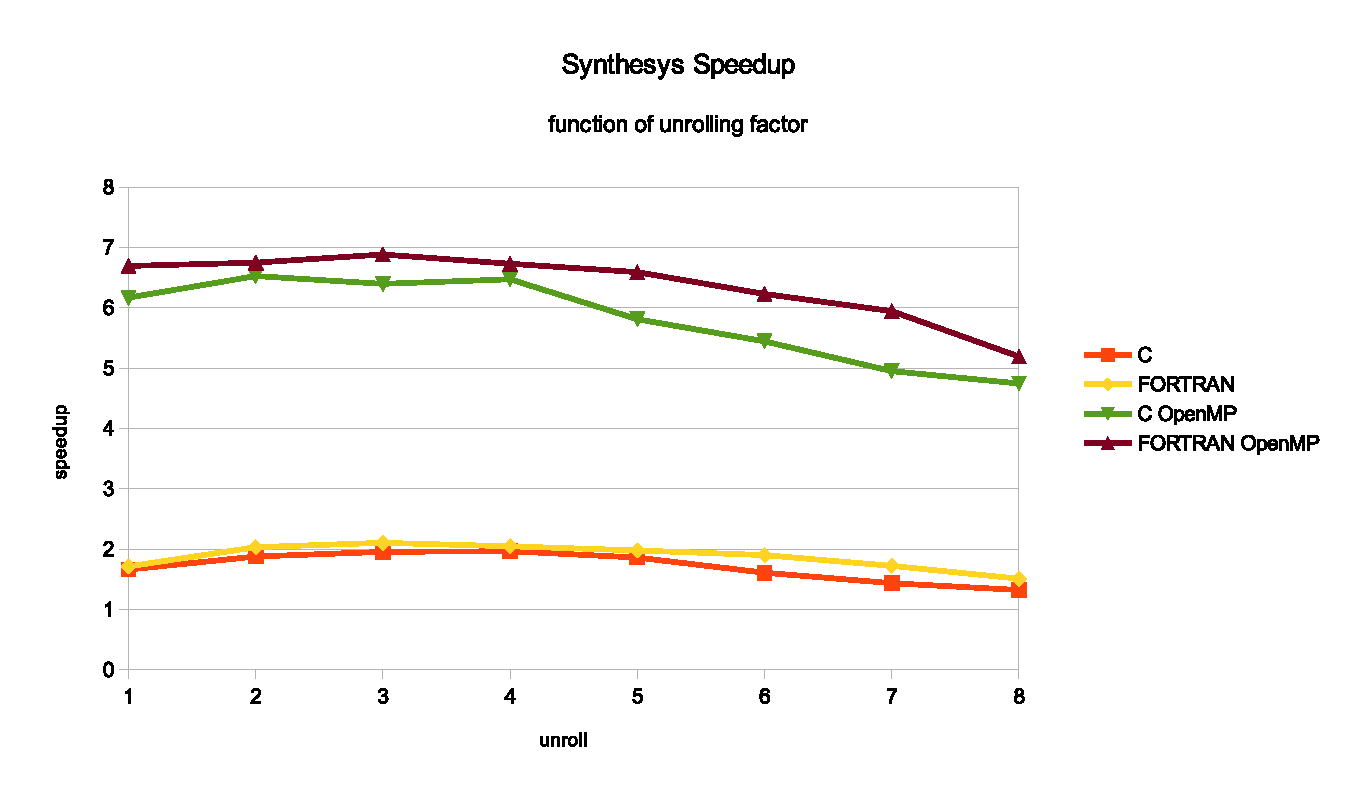
\includegraphics[scale=0.5]{Res_synthesis}\\


\end{frame}


\begin{frame}
\frametitle{Improvement for BigDFT}
\begin{itemize}
\item Most of the convolutions have been ported to BOAST.
\item Results are encouraging: on the hardware BigDFT was hand optimized for, convolutions gained on average between 30 and 40\% of performance.
\item MagicFilter OpenCL versions tailored for problem size by BOAST gain 10 to 20\% of performance.
\end{itemize}
\end{frame}

\begin{frame}
\frametitle{SPECFEM3D OpenCL port}
Fully ported to OpenCL with comparable performances (using the \texttt{global\_s362ani\_small} test case):
\begin{itemize}
\item On a 2*6 cores (E5-2630) machine with 2 K40, using 12 MPI processes:
\begin{itemize}
\item OpenCL: 4m15s
\item CUDA: 3m10s
\end{itemize}
\item On an 2*4 cores (E5620) with a K20 using 6 MPI processes:
\begin{itemize}
\item OpenCL: 12m47s
\item CUDA: 11m23s
\end{itemize}
\end{itemize}
Difference comes from the capacity of cuda to specify the minimum number of blocks to launch on a multiprocessor.
Less than 4000 lines of BOAST code (7500 lines of cuda originally).
\end{frame}

\section{Conclusions and Future Work}

\begin{frame}
\frametitle{Conclusions and Future Work}
\end{frame}

\begin{frame}
\frametitle{Conclusions}
Generator has been used to test several loop unrolling strategies in BigDFT.\\
Highlights:
\begin{itemize}
\item Several output languages.
\item All constraints have been met.
\item Automatic benchmarking framework allows us to test several optimization levels and compilers.
\item Automatic non regression testing.
\item Several algorithmically different versions can be generated (changing the filter, boundary conditions...).
\end{itemize}
\end{frame}

\begin{frame}
\frametitle{Future Works and Considerations}
Future work:
\begin{itemize}
\item Produce an autotuning convolution library.
\item Implement a parametric space explorer or use an existing one (ASK: Adaptative Sampling Kit, Collective Mind...).
\item Vector code is supported, but needs improvements.
\item Test the OpenCL version of SPECFEM3D on the Mont-Blanc prototype.
\end{itemize}
Question raised:
\begin{itemize}
\item Is this approach extensible enough?
\item Can we improve the language used further?
\end{itemize}

\end{frame}



\end{document}
